%----------------------------------------------------%
%                     CONCLUSIONES                   %
%----------------------------------------------------%

\pagestyle{fancy}

\chapter{Conclusiones y Líneas futuras}
\label{conclusiones}

\textit{\textbf{exerClick}} es la aplicación para el seguimiento de ejercicios en el aula desarrollada en este proyecto. Su objetivo principal es dar una visión más real de lo que hacen los alumnos (tanto una visión global del grupo como individual), de modo que el docente pueda ofrecer un aprendizaje más adaptado e individualizado, aunque los grupos de alumnos sean muy grandes.\\

Se planteó al inicio como una aplicación web, al igual que su antecesor, qClick \cite{qclick}, una aplicación de pregunta-respuesta en un entorno docente. Se decidió cambiar a una aplicación móvil finalmente, conllevando el cambio en la tecnología principal: \textit{Apache Cordova}. Las tecnologías principales (tecnologías web) se mantuvieron intactas gracias a Cordova: HTML5, CSS3 y Javascript. Ésto permitió realizar una aplicación móvil manteniendo las tecnologías acordadas al inicio del proyecto.\\

El proyecto partió de algo sencillo como idea inicial (objetivo de las primeras iteraciones): una aplicación sencilla de lanzar un ejercicio simple, que el alumno envíe su \textit{feedback} (el estado en el que se encuentra su ejercicio) y el profesor pueda visualizar esa respuesta (tanto de forma individual como grupal, aportando una visión global). Sin embargo, durante la captura de requisitos inicial se vio que había muchas ideas sobre la mesa que podrían ser interesantes, algunas descartadas por requerir quizá demasiado tiempo o ser demasiado ambiciosas. Esto, aun así, aportó gran inspiración para el desarrollo de la aplicación, pudiendo añadir más funcionalidad de forma incremental.\\

El proyecto fue lento al principio debido a la obligación del aprendizaje de la tecnología \textit{Apache Cordova} (y la adaptación de ésta a móviles) y Responsive Web Design. En esta etapa se intentó perfeccionar el objetivo más básico de lanzar un ejercicio, especialmente su interfaz, que había que adaptar muy bien a móviles. Se quería crear también algo reutilizable, de modo que las siguientes interfaces fueran más sencillas de crear. Esto creo un \textit{boom} importante en las fases finales del proyecto, donde se consiguieron crear muchas interfaces y cumplir muchos objetivos en un corto periodo de tiempo.\\

Desde el inicio del proyecto se pensó en tener alumnos evaluando la aplicación, dando un \textit{feedback} más cercano y constante. Debido a lo tarde que apareció una versión útil de la aplicación (que los usuarios pudieran manejar) los alumnos no probaron la aplicación hasta fechas tardías. Incluso hasta poder generar el fichero APK sólo se hicieron pruebas en un único móvil en el que estaba instalada la aplicación (en el anexo \ref{anexo-b} se pueden ver los resultados de esa prueba). Después se les pasó el fichero APK para poder probarla en sus propios móviles, de cara a ver como se adaptaba la aplicación a diferentes dispositivos y de tener un \textit{feedback} más continuo. En este punto no se llevaron acabo evaluaciones presenciales, sólo se recibían opiniones de pruebas por petición del autor o por iniciativa propia de los alumnos. Pese a que no se llevó acabo como fue planeado, las aportaciones recibidas por los usuarios fueron vitales para ciertos errores o para mejorar aspectos importantes de la aplicación.\\

\section{Objetivos alcanzados}

Como se ha comentado, hubo muchas ideas descartadas al inicio por ser demasiado ambiciosas o salirse del alcance previsto del proyecto. Entre los objetivos seleccionados, se han conseguido llevar a cabo satisfactoriamente todos excepto uno, que se comenta en el apartado \ref{step0:uos}.\\

\textbf{Objetivos del Alumno}\\

\textbf{UO1-S:} \textit{Responder a un ejercicio.} El alumno quiere indicar que ha acabado o que tiene dudas con un ejercicio que el profesor ha propuesto. Para ello, se ha pensado en que el alumno puede marcar el ejercicio con uno de los dos estados. A modo de \textit{feedback}, el profesor recibirá el estado (acabado o con dudas) de ese alumno.\\

\textbf{UO2-S:} \textit{Ver detalles de un ejercicio.} El alumno quiere ver más detalles sobre un ejercicio disponible y activo en la sesión. Al pinchar sobre un ejercicio puede ver cualquier detalle extra que el profesor haya decidido añadir.\\

\textbf{Objetivos del Profesor}\\

\textbf{UO1-T:} \textit{Crear-Lanzar un ejercicio simple.} El profesor quiere proponer un ejercicio rápidamente, sin escribir mucho. Ésto resulta especialmente útil cuando se tiene claro cuales son los ejercicios que se mencionan (se sabe el tema, la página... el contexto de qué ejercicios se están realizando es claro) y cuando se quieren lanzar rápidamente sin perder mucho tiempo.\\

\textbf{UO2-T:} \textit{Crear-Lanzar un ejercicio detallado.} El profesor quiere proponer la realización de un ejercicio preparado previamente o con bastantes detalles. Al contrario que en el UO1-T, en este caso el profesor se los puede preparar fuera de una sesión, incluso llegando a inventarse un ejercicio.\\

\textbf{UO3-T:} \textit{Cambiar el tipo de ejercicio.} El profesor desea cambiar un ejercicio del tipo que tiene a otro cualquiera (de activo a finalizado, por ejemplo). Fundamental cuando se desea lanzar un ejercicio que estaba guardado mientras se preparaba mejor, cuando queremos dar un ejercicio por finalizado o cuando nos confundimos en cualquier cambio y queremos deshacerlo.\\

\textbf{UO4-T:} \textit{El profesor desea ver qué tal le ha ido a la clase en general o a un alumno en un ejercicio.} Este UO es quizá de los más importantes, ya que es el que nos muestra todo el \textit{feedback} recibido de los alumnos. Podemos ver el estado de un ejercicio para cada alumno o ver globalmente (en porcentajes) el progreso de la clase.\\

\textbf{UO5-T:} \textit{Ver la descripción completa de un ejercicio.} Un profesor quiere ver la descripción completa de un ejercicio (identificador, enunciado, página, tema, etc.).\\

\textbf{UO6-T:} \textit{Editar un ejercicio.} El profesor desea editar los atributos de un ejercicio. Quizá se haya equivocado al crear el ejercicio en algún detalle o quiera añadir más detalles. Especialmente útil para los ejercicios que se han guardado y se quieren preparar mejor.\\

\textbf{UO8-T:} \textit{Cerrar sesión.} El profesor quiere cerrar su sesión activa.\\

\textbf{UO9-T:} \textit{Cambiar el idioma de la aplicación.} El profesor desea cambiar el idioma con el que lee la aplicación. Un requisito fundamental de cara a la internacionalización fue que la aplicación estuviera en 4 idiomas: castellano, euskera, inglés y francés.\\

\textbf{UO10-T:} \textit{Cambiar de asignatura.} El profesor, que tiene más de una asignatura, quiere cambiar de una asignatura x a otra asignatura y.\\

\section{Líneas futuras y Propuestas de mejora}

\textit{\textbf{exerClick}} fue pensada como parte de un proyecto mayor, \textit{pClick} y a su vez \textit{PresenceClick}, que integrará ésta y otras aplicaciones. Pasaría a tener un módulo en \textit{PresenceClick}, de modo que algunas opciones de \textit{\textbf{exerClick}} que quizá necesiten de un entorno de trabajo más apropiado (como un ordenador) podrían exportarse a ese módulo.\\

Además de ésto, se pensaron más ideas relacionadas a \textit{\textbf{exerClick}} que quedaron en el tintero. La siguiente lista aporta todas esas ideas y otras que surgieron durante o después del desarrollo del proyecto:

\begin{itemize}
\item Evaluar a un alumno en un ejercicio (UO7-T). Este objetivo se marcó como una posibilidad y resultaba interesante. Para un ejercicio se permitía asignarle a un alumno una valoración del 1 al 5 (usando \textit{emoticonos} de tristeza o sonrisa de diferentes grados) al igual que hace \textit{PresenceClick}. El docente se acercaría a un alumno, vería el estado en el que se encuentra con el ejercicio y si al docente le pareciera correcto podría darle una valoración (no visible para el alumno, es algo personal del docente).\\

Otro objetivo diferente sería que el propio alumno pudiera valorarse a si mismo, de modo que cuando un profesor da un ejercicio por finalizado el alumno puede introducir una valoración sobre si mismo.\\

\item Mejorar la autenticación queda abierta para varias mejoras:
\begin{itemize}
\item Mejorar el control de errores como que no haya conexión (con un aviso), por ejemplo.
\item Que a un alumno se le reconozca si se ha identificado en la clase (utilizando el sistema de reconocimiento por tarjeta) y en caso contrario enviar un mensaje de error.
\end{itemize}

\item Poder descargar un PDF con los detalles de los ejercicios, de modo que para ejercicios con muchos detalles se tuviera una visualización más sencilla.

\item Borrar ejercicios por completo. Esta idea se pensó en realizarla desde PresenceClick por seguridad, por eso no se ha implementado.

\item Permitirle al alumno acceder a su propio perfil con las posibilidades de cerrar sesión y cambiar de idioma (al igual que el profesor). Debido a la semejanza entre pantallas no llevaría mucho trabajo añadir esta mejora.

\item Mejorar el uso de Responsive Web Design en pantallas grandes. Se ha usado RWD para adaptar el diseño a cualquier pantalla, enfocándose en una pantalla de un dispositivo móvil. En tablets, por ejemplo, el diseño deja muchos huecos libres sin aprovecharse. Sería interesante aprovechar esos espacios libres para añadir más información. También se podría plantear el diseño de otra manera para aprovechar mejor las pantallas grandes. 
\end{itemize}

Toda la información reunida con exerClick que alimente la base de datos proporcionará datos muy interesantes para futuros usos. Si bien por si sola la información de exerClick no parece demasiado útil, una vez que juntemos esta y la información reunida por los otros módulos tendremos una base de datos con muchísima información para realizar todo tipo de procesos. Podríamos realizar incluso predicciones sobre el rendimiento de los alumnos hacia el final del curso, por ejemplo (lo que viene siendo \textit{Machine Learning}). Se puede usar la información para ver como se podría mejorar una asignatura respecto a entregables, clases, etc. Hay bastantes posibilidades futuras, pero \textit{\textbf{exerClick}} se dejó en este punto como un Trabajo de Fin de Grado, con posibilidades de mejora hacia el futuro.\\

\section{Lecciones aprendidas}

\subsection*{Apache Cordova vs Aplicación Nativa}
\begin{itemize}
\item Basándome en mi experiencia durante el proyecto y en algunas opiniones recogidas me ha parecido que la tecnología de Apache Cordova intenta abarcar demasiado. Las aplicaciones que se generan se vuelven lentas y con fallos. Para un proyecto que quiera un diseño interesante, sin embargo, Cordova es una herramienta sencilla de usar. También para aquellos que no tengan conocimientos de las tecnologías de Android y quieran crear una aplicación esta herramienta es estupenda.\\

Para desarrollar una futura aplicación, en lo personal, tendría en cuenta crear una aplicación nativa de Android. El desarrollo de la interfaz ha sido la parte más costosa de esta aplicación, cosa que con una aplicación nativa es sencillo y robusto, adaptable a cualquier pantalla fácilmente (con Cordova hay que romperse más la cabeza). A parte de eso señalaría también los siguientes motivos:
\begin{itemize}
\item La falta de documentación de Cordova frente a al gran comunidad de Android.
\item Gestores de errores o \textit{plugins} fáciles de instalar y utilizar en Android con Cordova se vuelven una pesadilla.
\end{itemize}
En resumen, escoge Cordova si:
\begin{itemize}
\item No tienes conocimientos de Android.
\item Quieres realizar una aplicación visualmente atractiva con tus conocimientos web.
\item La aplicación es ligera y no va a tener demasiada funcionalidad.
\end{itemize}
Y crea una aplicación nativa en Android si:
\begin{itemize}
\item Va a tener muchas funcionalidades.
\item Vas a manejar muchas animaciones o efectos.
\item Quieres crear algo simple (sin meterte en todo el tema Cordova) o algo realmente amplio (resulta más cómodo para no tener tantos problemas).
\end{itemize}
\end{itemize}

\subsection*{Generar un apk con Apache Cordova}

Para generar un apk necesitaremos usar un IDE de desarrollo, en este caso se usó Eclipse Luna. Crearemos un nuevo proyecto en Android con el código que tenemos (si no estábamos trabajando ya sobre un IDE) tal y como se muestra en la figura \ref{fig:LLAA-1}.\\

\begin{figure}[!htbp]
	\centering
	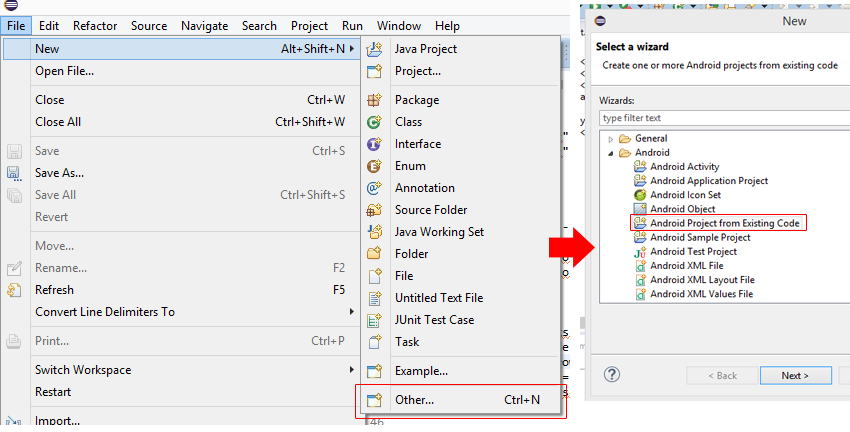
\includegraphics[width=\textwidth]{LLAA_1}
	\caption{Primer paso: crear un proyecto nuevo}
	\label{fig:LLAA-1}
\end{figure}

En el proyecto nuevo debemos meter nuestro código en la ruta ''\textit{assets/www}'' (si no existe cread las carpeta necesarias). También necesitaremos el archivo cordova.js que podemos conseguir en https://github.com/apache/cordova-js. Deberíamos tener algo parecido a la estructura de la figura \ref{fig:LLAA-2}.\\

\begin{figure}[!htbp]
	\centering
	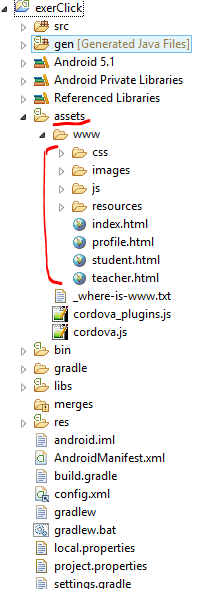
\includegraphics[height=10cm]{LLAA_2}
	\caption{Segundo paso: tener la estructura y archivos correctos}
	\label{fig:LLAA-2}
\end{figure}

Finalmente debemos ejecutar el proyecto (aunque no llegue a cargarse el emulador, para hacerlo rápido podemos anular el proceso cuando se nos pida escoger el emulador). Una vez ejecutado se habrá creado el apk y podremos encontrar en la carpeta bin de nuestro proyecto de Eclipse (figura \ref{fig:LLAA-2}).\\